\chapter{Discussion}

In this section, we provide several points of discussion for this study, including identifying the disconnection between  discussion on the potential improvement of the expertise model, and other data sources to include in order to fill the gap between cognitive research and expertise location studies in software engineering.

\section{``How Well Do They Perform'' v.s. ``What Have They Done''}

By reviewing our repository, we found the quantitative expertise model has been constantly evolving, which adds new data sources, such as adding interaction data \cite{fritz2010degree}, and including API usage data \cite{schuler2008mining} into their expertise measurement model. However, these expertise models still have failed to measure the cognitive characteristics of experts, which were identified by early cognitive studies \cite{MCKEITHEN1981307, Simon:1996:SA:237774, gobet1996recall}. Based on these previous researches, experts process, i.e., receive and recall, their domain information faster and more precisely, which grants their higher proficiency in their domains. The excellence of their information processing ability helps them to automatically realize the best solution and handle unexpected situation \cite{ericsson2006cambridge}. Conclusion from these cognitive studies is evidenced by empirical studies which monitoring the experts performance while doing the task (monitoring how well expert perform). However, the heavy experience-based expertise models (measuring what have expert done) fail to reflect developers ability in processing information in field of software engineering. We argue that there is a \textbf{disconnect} between early cognitive studies on expert performance and the software engineering approaches and systems for locating expertise, and over-rely on the experience based expertise model may bias the assessment of expertise. There is only a few studies that follow studies on building standards for evaluating the expertise level of a developer \cite{bergersen2014construction}, but to the best of our knowledge, we are not able to find a study that aims at automatically measuring and locating expertise by assessing the information processing ability of a developer rather than mining the their previous experience.

\section{Community Feedback v.s. Automated Expertise Location Techniques}

Employing human judgment to assess the expertise of a developer is normal practice while locating expertise \cite{mcdonald1998just}. For example, the approaches of ``\textit{everyday expertise}'' and ``\textit{expertise concierge}'' are employing human judgment to determine expertise \cite{mcdonald1998just}, it is common practice to rely a human to assess the expertise of developers especially considering acknowledgement from dignitaries in the community, and there is previous study to include feedback data into the expertise profile \cite{Reichling2007}. As the emergence of business and employment-oriented service sites such as Linkedin, it certifies the users' expertise based on the \textit{endorsement} from their peer in their connection circle and other Linkedin users \cite{linkedin}, and GitHub has popular repositories and site which rank followers\footnote{Following People, https://help.github.com/articles/following-people/} and stars\footnote{About Stars, https://help.github.com/articles/about-stars/} received from the community.

\begin{figure}
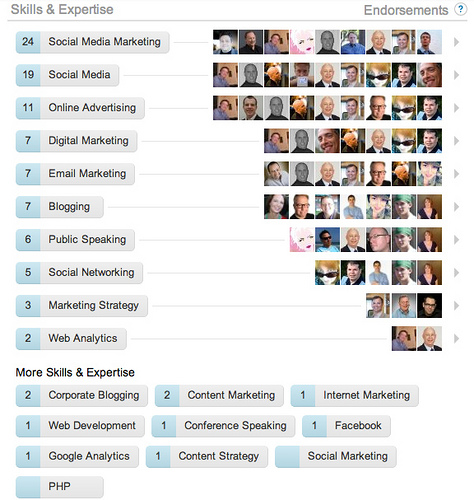
\includegraphics[width = 0.6\columnwidth]{linkedin-endorsements.jpg}
\centering
\caption{The Endorsement System in LinkedIn. A list of User Profile Pictures on the Right of Each ``Skills \& Expertise'', and Number on the Left Indicates How Many Connections in Their Social Network Have Certified This Item of Skill \cite{endorsement}.}
\label{endorsement}
\end{figure}

However, this type of evaluation for expertise can be very easily manipulated,  such as Twitter where users can purchase followers by number. In a previous study \cite{marlow2013activity}, user study participants have already mentioned that popularity is an indicator but not always enough to evaluate the quality of work. We argue the \textit{endorsement} on LinkedIn is also an indicator of popularity but on skills and expertise of a developer.

In the future study, we purpose to carefully integrate the user rating and popularity based expertise evaluation with the automated techniques which mostly just retrieve the activity history of a developer. However, we need to find a balance between employing user feedback and the historical data, but avoid over-reliance on the either single data source.

\section{Paradox of Expertise}

The ultimate goal of locating expert is to find someone for providing the qualified and effective performance for a job or task, and it is non-trivial to firstly determine the high-level goal of locating expertise. However, even if experts have experienced so much in the past, when it comes to certain task that requires to share expertise, such as training and coaching new employers, the person with highest expertise may not be the best candidate for performing these tasks due to the paradox of expertise \cite{dror2011paradox}, since they are biased by their own experience and capacity \cite{liu2013expertise}.

Experts think differently than novices, and their over average performance in information processing is based on a pre-determined and routine mechanism. This mechanism is highly effective, but also restricts the flexibility and control while expressing and articulating their specialties \cite{dror2011paradox}. For example, one of the best basketball players in the history, Michael Jordan, has never been a head coach of any basketball teams which, in fact, is determined by his extremely high motion expertise in basketball, and it restricts his expression for his drills in playing basketball game e.g., Michael may believe dunking basketball over his opponent is an easy task, which is biased opinion due to his superior athleticism \cite{staff_nba.com_2017}.

In the study of Dror \cite{dror2011paradox}, they claim one of the major reason causing this paradox is the heavy amount of training that expert has received. Once their formed an automated routine, their expertise is not easily accessible, and spending effort for accessing this effort degrades experts' performance \cite{flegal2008overthinking}. Therefore, expertise location studies need to consider this ``paradox'' of expert, and while locating expertise for expertise sharing tasks, novices may actually help experts to avoid this paradox. For example, \textit{Arthur Andersen LLP}\footnote{Arthur Andersen LLP was one of the largest accounting firm in the US} allocates their new hires called ``green beans'', into expert teams \cite{greenbeans}. These ``green beans'' ask basic questions such as definition of terminologies, which helps the experts access their expertise when green beans asking questions \cite{kelly2009leadership}.

\section{Guiding Entry-level Novices}

Conventional expertise location techniques are usually employed in recommending people for performing specific software engineering task, and also in hiring, training and allocating software talents \cite{bergersen2014construction}. However, as open source software is playing an important role in the software industry,  and due to its voluntary attribute \cite{shah2006motivation}, it is non-trivial to guide and encourage more participants to the community. However, newcomers of open source projects are facing various heavy barriers to enter the community.

Past research by \citeauthor{STEINMACHER201567} has identified five main categories of these barriers \cite{STEINMACHER201567}. The major categories of these barriers are:

\begin{itemize}
    \item \textit{Technical Hurdles}: difficulties in understanding the code or setting up the work space and environment.
    \item \textit{Documentation}: difficulties in understanding the project.
    \item \textit{Social interactions}: communication issues with the previous contributors of the project.
    \item \textit{Newcomers previous knowledge and expertise}: similar to technical hurdles, but more focusing on the newcomer's own technical expertise such as experience in software engineering practice.
    \item \textit{Starting point}: difficulties in finding a mentor or entry level task to start.
\end{itemize}

Except the difficulty in social interaction, other barriers can be addressed or alleviated by mature expertise location systems, particular finding a mentor with required expertise to guide or help the novice to perform the technical task \cite{begel2008novice}. Further, in order to support newcomers to find the available expertise in the project and then enter the community for contribution, it also shows the non-trivial requirement of the expertise location systems which is including the constraints of the others such as their availability.

% do not use awareness information for constraints

% "disconnect" gap between doing it and what have done
\section{Limitations}

In this study, we reviewed the expertise location approaches and systems in Software Engineering and Computer Supported Collaborative Work based on our research questions. However, during our research procedure, we found early cognitive studies on are not only focused and limited in the field of Software Engineering. Though there are early studies about the relation between the information processing ability and programming expertise in the software engineering practice, we are not able to locate any studies that aimed to systematically build theories for measuring the expertise level for software engineering personnel. Due to the scope of this study, we only focus the papers in the field of Software Engineering and Computer Supported Collaborative Work, we may miss the progress in cognitive studies which analyze expert behaviors and characteristics. In the future study, we also intend to explore studies from other research subjects other than these two we have already reviewed in this study, particularly for field in management, organizational and cognitive science. In addition, we find related literature is not limited in the form of paper publications. There are lots of valuable resources in books \cite{ericsson2006cambridge, Simon:1996:SA:237774}, and we intend to include these resources as well.